\begin{frame}
\frametitle{Separation of Concerns}
\begin{block}{Different expertise, different focus}
Relevant pieces of code should be easy to divide
\end{block}
\begin{itemize}
\item Much like any library -- clients control behavior by passing
  arguments, not modifying implementation
\item Can be very flexible -- arguments with behavior of their own
  (e.g., functors)
\item Several examples: initial mapping schemes, dynamic load
  balancing strategies
\item CS-specialist logic doesn't pollute application code, can be
  swapped out with minimal effort
\item Location-independent algorithm expression and runtime-mediated
  execution are essential enabling features
\end{itemize}
\end{frame}


\begin{frame}
\frametitle{Different expertise, different focus}
\framesubtitle{Mapping Example: Quantum Chemistry with {\sc OpenAtom}}
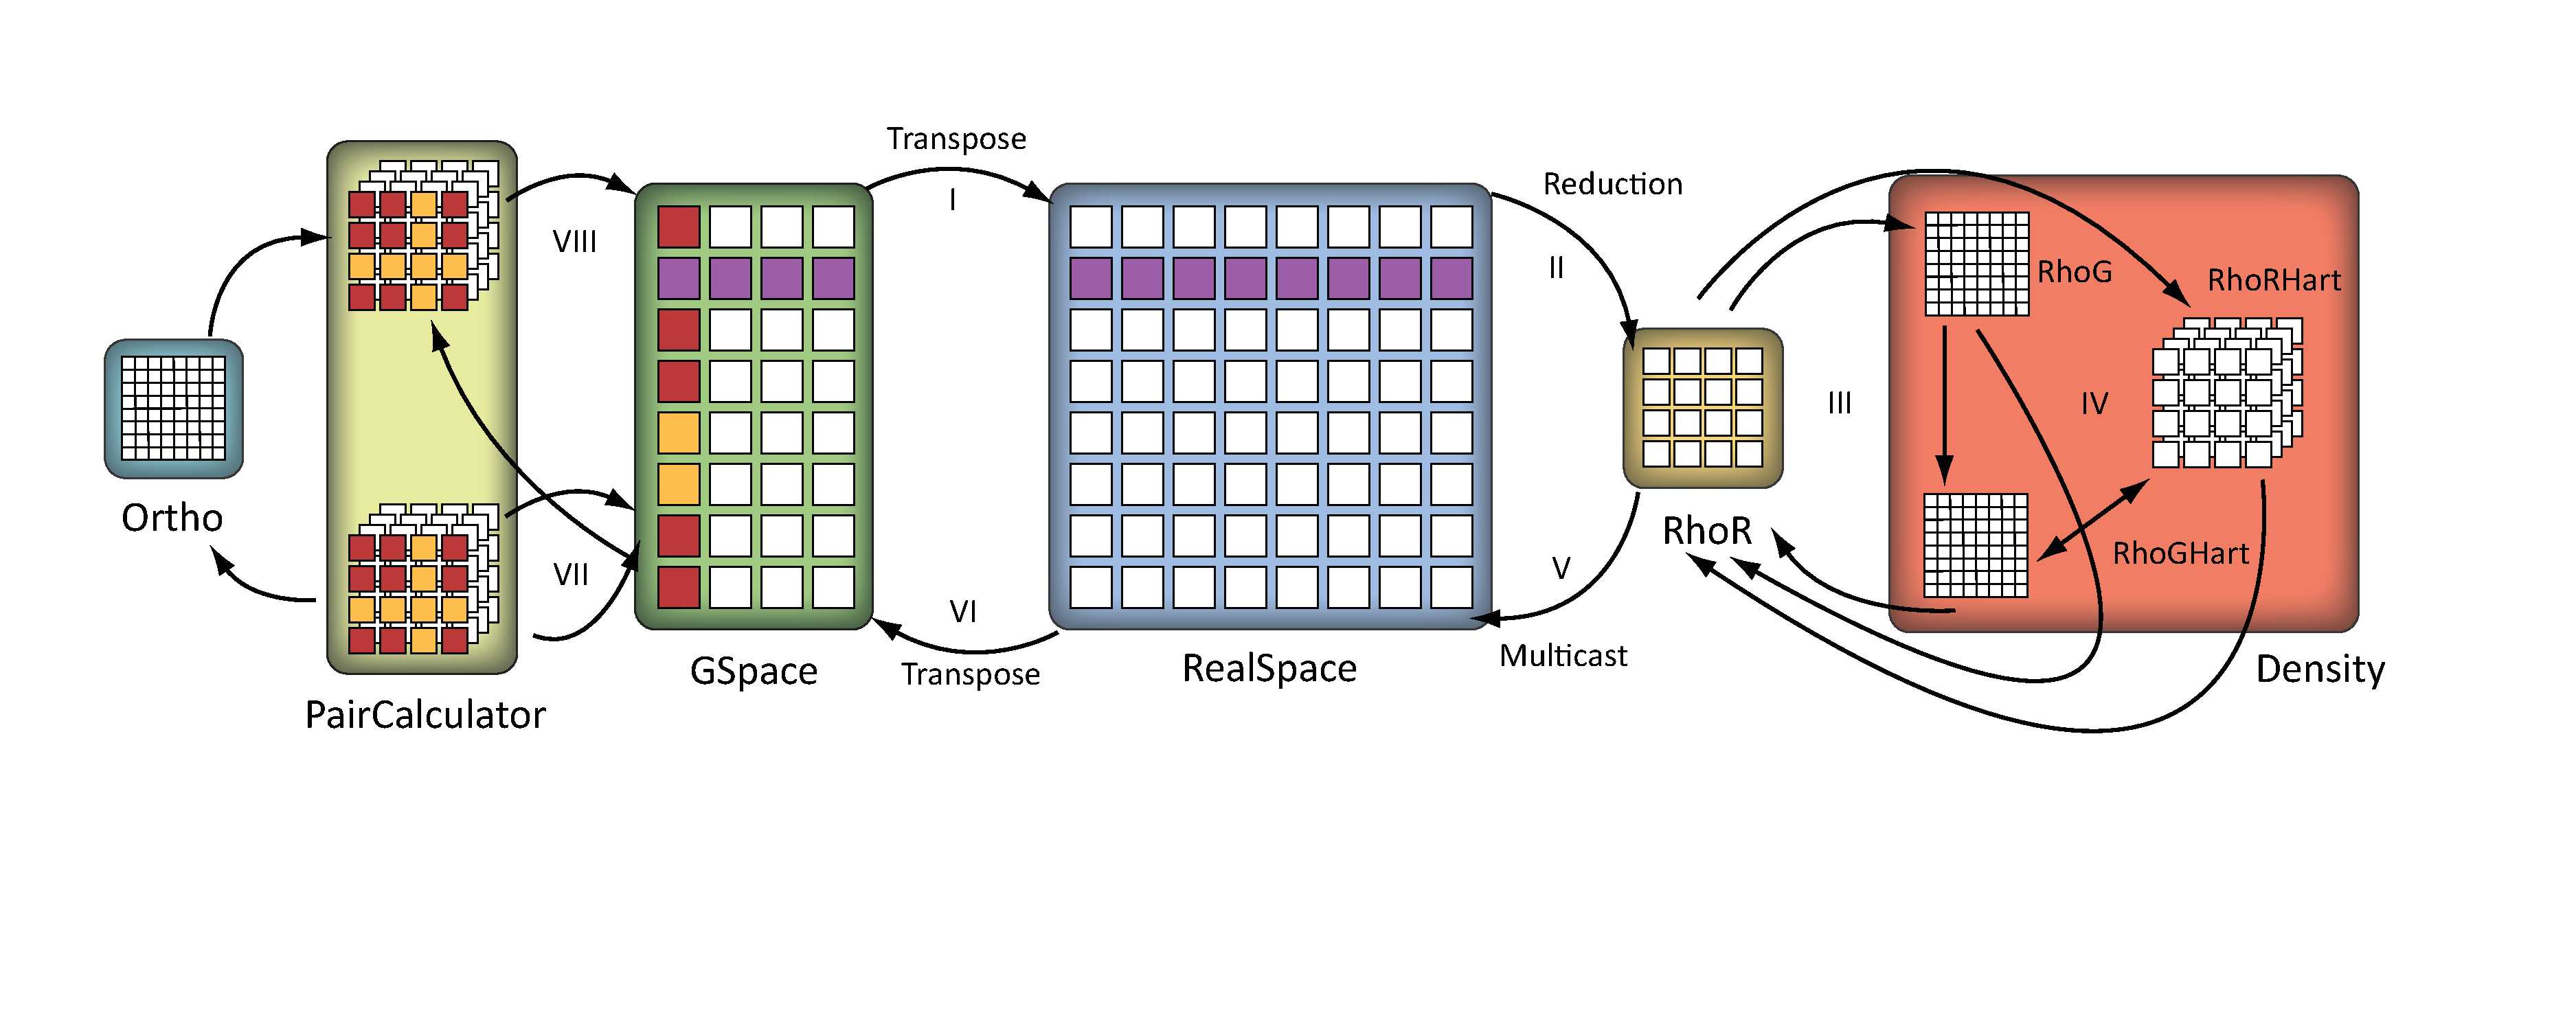
\includegraphics[width=\textwidth]{../figures/openatom/control-flow.pdf}
\end{frame}

\begin{frame}
\frametitle{Different expertise, different focus}
\framesubtitle{Mapping Example: Quantum Chemistry with {\sc OpenAtom}}
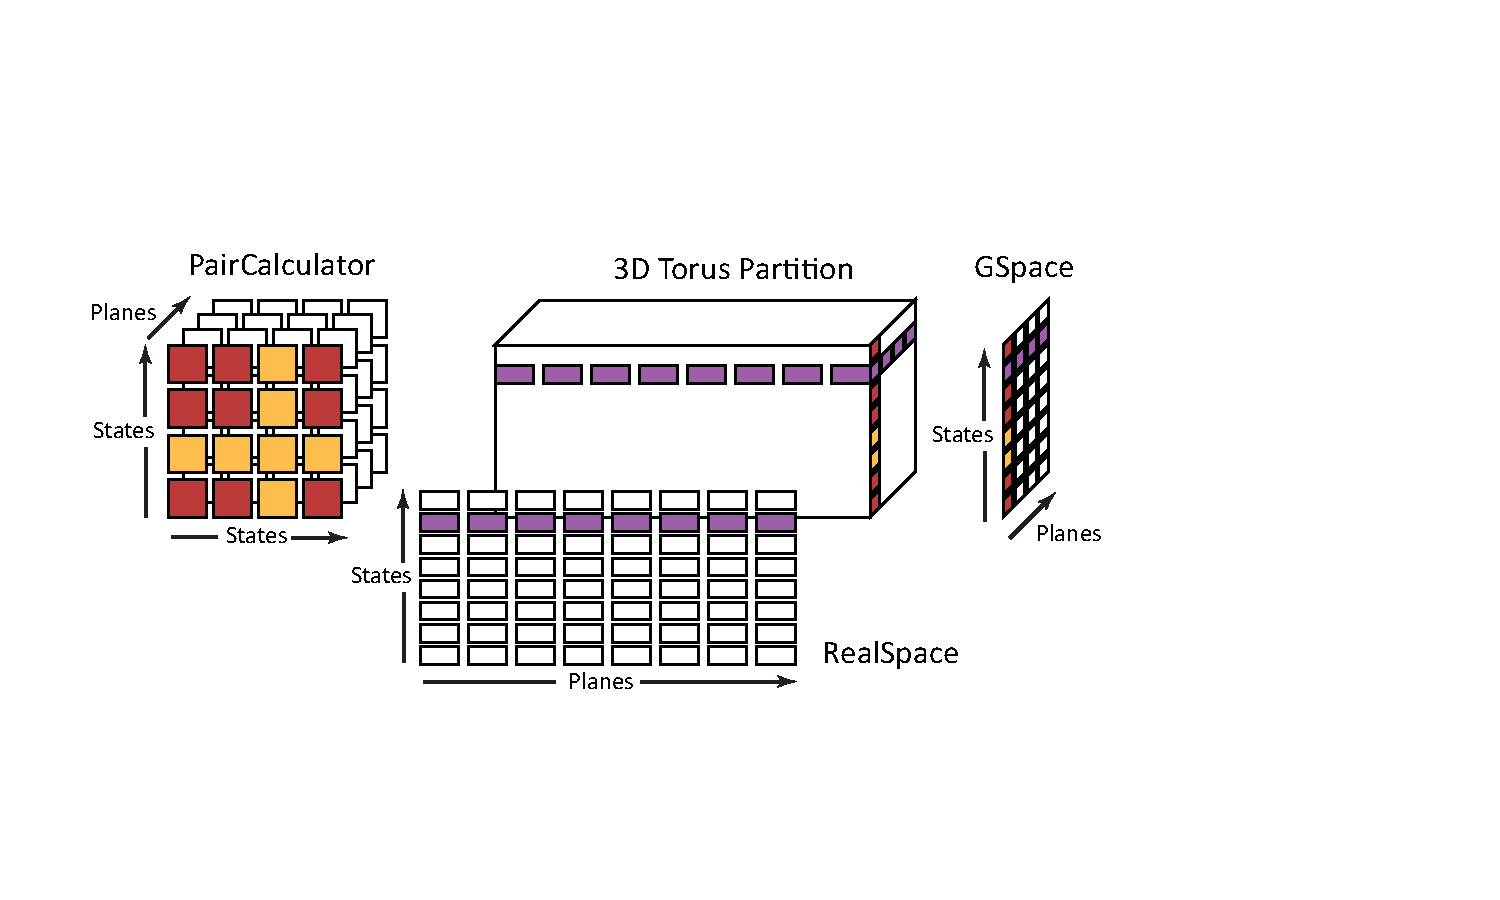
\includegraphics[width=0.9\textheight]{../figures/openatom/mapping.pdf}
\end{frame}


\begin{frame}
\frametitle{Different expertise, different focus}
\framesubtitle{Mapping Example: Quantum Chemistry with {\sc OpenAtom}}
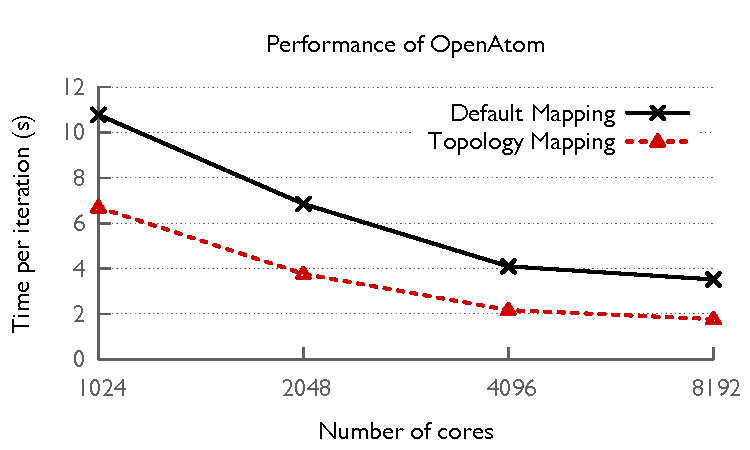
\includegraphics[width=0.9\textwidth]{../figures/openatom/map.pdf}
\begin{block}{40\% improvement, application only changed in initialization!}\end{block}
\end{frame}


\begin{frame}
\frametitle{Separation of Concerns}
\begin{block}{Layered responsibility}
Application worries about \emph{what}, runtime system worries about \emph{how}
\end{block}
\begin{itemize}
\item What data to send, vs. message allocation and packing
\item Who to talk to, vs. where they live
\end{itemize}
\end{frame}

\begin{frame}[t]
\frametitle{Separation of Concerns}
\framesubtitle{Example: Object location services}
\begin{itemize}[<+->]
\item Possible solutions to ``Where does object X live?''
\begin{itemize}[<+->]
\item Name is location-specific
\item Object creator specifies location, passes along with name
\item Fixed mapping from names to locations
\item \textbf{Dynamic lookup}
\end{itemize}
\item \charm approach
\begin{itemize}
\item \emph{Mapping scheme} defines \emph{home location} -- default location, and responsible for knowing current location
\item Cache of last known locations on each processor
\item Messages sent to cached location, or home if none known
\end{itemize}
\end{itemize}
\pause
\begin{block}{Application is mostly oblivioous}
Fire off message, runtime delivers
\end{block}
\end{frame}

\begin{frame}
\frametitle{Separation of Concerns: Object Migration}
\begin{block}{Why migrate?}
\begin{itemize}
\item Fault tolerance
\item Communication locality
\item Load balance
\item Power, Energy, and Heat management
\end{itemize}
\end{block}
\pause
Application provides serialization routines, runtime can do the rest!
\end{frame}

\begin{frame}[fragile]
\frametitle{Object Serialization}
\begin{columns}
\begin{column}{0.5\textwidth}
\begin{lstlisting}
class MyChare : public CBase_MyChare {
  int a;   float b;   char c;
  float localArray[LOCAL_SIZE];
  int heapArraySize;
  float* heapArray;
  MyClass *pointer;
  // . . . 
};
\end{lstlisting}
\end{column}
\begin{column}{0.5\textwidth}
\begin{lstlisting}
void MyChare::pup(PUP::er &p) {
   CBase_MyChare::pup(p);
   p | a;  p | b; p | c;
   p(localArray, LOCAL_SIZE);
   p | heapArraySize;
   if (p.isUnpacking()) {
     heapArray =
       new float[heapArraySize];
   }
   p(heapArray, heapArraySize);
   bool isNull = pointer==NULL;
   p | isNull;
   if (!isNull) {
     if (p.isUnpacking())
       pointer = new MyClass();
     p | *pointer;
   }
}
\end{lstlisting}
\end{column}
\end{columns}
\end{frame}
